% Foliensatz: "AFu-Kurs nach DJ4UF" von DK0TU, Amateurfunkgruppe der TU Berlin
% Lizenz: CC BY-NC-SA 3.0 de (http://creativecommons.org/licenses/by-nc-sa/3.0/de/)
% Autoren: Martin Deutschmann <martin.deutschmann@campus.tu-berlin.de>
% Korrekturen: Lars Weiler <dc4lw@darc.de>, Sebastian Lange <dl7bst@dk0tu.de>

\documentclass[aspectratio=169]{beamer}

\usepackage[ngerman]{babel} % deutsche Worttrennung etc.
\usepackage[utf8]{inputenc} % UTF8 Text

\usepackage[super, comma, numbers, square, sort]{natbib}

\usepackage{hyperref}       % Hyperref Package für bessere Referenzen (todo)
\hypersetup{
	colorlinks=false,       %   false: boxed links; true: colored links
    %linkcolor=white,       %   color of internal links (change box color with linkbordercolor)
    citecolor=red,          %   color of links to bibliography
    filecolor=white,        %   color of file links
    urlcolor=blue           %   color of external links
}

\usepackage{multirow}
\usepackage{wasysym}  % Math Symbols like \permil
%\usepackage{colortbl}
%\usepackage{subscript}
%\usepackage{caption}
%\usepackage{setspace}
%\usepackage{xcolor}        % benutze CodeListe

% Footnote
%\usepackage{hanging}
%
%\setbeamertemplate{footnote}{%
%  \hangpara{2em}{1}%
%  \makebox[2em][l]{\insertfootnotemark}\footnotesize\insertfootnotetext\par%
%}


%\usepackage{pgf}
%\usepackage{tikz}
%\usetikzlibrary{arrows,automata}
%\usetikzlibrary{positioning}
%
%\tikzset{
%    state/.style={
%           rectangle,
%           rounded corners,
%           draw=black, very thick,
%           minimum height=2em,
%           minimum width=2pt,
%           inner sep=2pt,
%           text centered,
%           },
%}

%\usepackage{listings}
%\lstset{basicstyle=\small, numberstyle=\tiny, extendedchars=true, numbers=left, numbersep=5pt}
%\lstset{showtabs=false, showspaces=false, showstringspaces=false}
%%\lstset{backgroundcolor=\color{white!75!lightgray}, , frame=single}
%%\lstset{backgroundcolor=\color{white}}
%%\lstset{backgroundcolor=none}
%\lstset{keywordstyle=\color{blue!50!gray},  identifierstyle=\color{black}}
%\lstset{commentstyle=\color{green!50!gray}, stringstyle=\color{red!50!gray}}
%\lstset{language=C, fontadjust=true, tabsize=2, breaklines=true}
%\lstset{backgroundcolor=\color{white!75!lightgray}, caption=\lstname, frame=single}
%\lstset{emphstyle=\color{black}\fbox}
%
%% Keine "Listing:"-Caption
%\captionsetup{labelformat=empty,labelsep=none}
%
%% für mathematische Umgebungen
%\usepackage{amsmath,amsfonts,amssymb}
%
%\lstdefinestyle{Bash}{
%language=Bash,
%frame=single,
%rulecolor=\color{black},
%backgroundcolor=\color{gray!50},
%keywordstyle=\color{black},
%identifierstyle=,
%commentstyle=\color{black},
%stringstyle=\color{magenta!65!white},
%showstringspaces=false,
%basicstyle=\footnotesize\ttfamily\color{black},
%numbers=none,
%breaklines=true,
%captionpos=b
%}

%\usepackage{listings}
%
%\lstdefinestyle{basic}{
%    captionpos=t,%
%    basicstyle=\footnotesize\ttfamily,%
%    numberstyle=\tiny,%
%    numbers=left,%
%    stepnumber=1,%
%    frame=single,%
%    showspaces=false,%
%    showstringspaces=false,%
%    showtabs=false,%
%    %
%    keywordstyle=\color{blue},%
%    identifierstyle=,%
%    commentstyle=\color{gray},%
%    stringstyle=\color{magenta}%
%}



% fließende Boxen haben keinen Abstand
%\fboxsep0mm

% inkludiere Creative Commons Helper
%%%%%%%%%%%%%%%%%%%%%%%%%%%%%%%%%%%%%%%%%%%%%%%%%%%%%%%%%%%%%%%%
%% ccBeamer 0.1, 2007-07-02                                   %%
%% Written by Sebastian Pipping <webmaster@hartwork.org>      %%
%% ---------------------------------------------------------- %%
%% Licensed under Creative Commons Attribution-ShareAlike 3.0 %%
%% http://creativecommons.org/licenses/by-sa/3.0/             %%
%%%%%%%%%%%%%%%%%%%%%%%%%%%%%%%%%%%%%%%%%%%%%%%%%%%%%%%%%%%%%%%%


%% Images
\newcommand{\CcImageBy}[1]{%
	
\includegraphics[scale=#1]{texdata/creative_commons/cc_by_30.pdf}%
}
\newcommand{\CcImageCc}[1]{%
	
\includegraphics[scale=#1]{texdata/creative_commons/cc_cc_30.pdf}%
}
\newcommand{\CcImageDevNations}[1]{%
	
\includegraphics[scale=#1]{texdata/creative_commons/cc_dev_nations_30.pdf}%
}
\newcommand{\CcImageNc}[1]{%
	
\includegraphics[scale=#1]{texdata/creative_commons/cc_nc_30.pdf}%
}
\newcommand{\CcImageNd}[1]{%
	
\includegraphics[scale=#1]{texdata/creative_commons/cc_nd_30.pdf}%
}
\newcommand{\CcImagePd}[1]{%
	
\includegraphics[scale=#1]{texdata/creative_commons/cc_pd_30.pdf}%
}
\newcommand{\CcImageSa}[1]{%
	
\includegraphics[scale=#1]{texdata/creative_commons/cc_sa_30.pdf}%
}
\newcommand{\CcImageSampling}[1]{%
	
\includegraphics[scale=#1]{texdata/creative_commons/cc_sampling_30.pdf}%
}
\newcommand{\CcImageSamplingPlus}[1]{%
	
\includegraphics[scale=#1]{texdata/creative_commons/cc_sampling_plus_30.pdf}%
}


%% Groups
\newcommand{\CcGroupBy}[2]{% zoom, gap
	\CcImageCc{#1}\hspace*{#2}\CcImageBy{#1}%
}
\newcommand{\CcGroupByNc}[2]{% zoom, gap
	\CcImageCc{#1}\hspace*{#2}\CcImageBy{#1}\hspace*{#2}\CcImageNc{#1}%
}
\newcommand{\CcGroupByNcNd}[2]{% zoom, gap
	\CcImageCc{#1}\hspace*{#2}\CcImageBy{#1}\hspace*{#2}\CcImageNc{#1}\hspace*{#2}\CcImageNd{#1}%
}
\newcommand{\CcGroupByNcSa}[2]{% zoom, gap
	\CcImageCc{#1}\hspace*{#2}\CcImageBy{#1}\hspace*{#2}\CcImageNc{#1}\hspace*{#2}\CcImageSa{#1}%
}
\newcommand{\CcGroupByNd}[2]{% zoom, gap
	\CcImageCc{#1}\hspace*{#2}\CcImageBy{#1}\hspace*{#2}\CcImageNd{#1}%
}
\newcommand{\CcGroupBySa}[2]{% zoom, gap
	\CcImageCc{#1}\hspace*{#2}\CcImageBy{#1}\hspace*{#2}\CcImageSa{#1}%
}
\newcommand{\CcGroupDevNations}[2]{% zoom, gap
	\CcImageCc{#1}\hspace*{#2}\CcImageDevNations{#1}%
}
\newcommand{\CcGroupNcSampling}[2]{% zoom, gap
	\CcImageCc{#1}\hspace*{#2}\CcImageNc{#1}\hspace*{#2}\CcImageSampling{#1}%
}
\newcommand{\CcGroupPd}[1]{% zoom
	\CcImagePd{#1}%
}
\newcommand{\CcGroupSampling}[1]{% zoom
	\CcImageSampling{#1}%
}
\newcommand{\CcGroupSamplingPlus}[1]{% zoom
	\CcImageSamplingPlus{#1}%
}


%% Text
\newcommand{\CcLongnameBy}{Attribution}
\newcommand{\CcLongnameByNc}{Attribution-NonCommercial}
\newcommand{\CcLongnameByNcNd}{Attribution-NoDerivs}
\newcommand{\CcLongnameByNcSa}{Attribution-NonCommercial-ShareAlike}
\newcommand{\CcLongnameByNd}{Attribution-NoDerivs}
\newcommand{\CcLongnameBySa}{Attribution-ShareAlike}

\newcommand{\CcNote}[1]{% longname
	This work is licensed under the \textit{Creative Commons #1 3.0 License}.%
}


% generelles Thema auswählen
\usetheme{Goettingen} %Berlin spart ohne Sidebar allerdings angenehm Platz
% AnnArbor | Antibes | Bergen | Berkeley | Berlin | Boadilla | boxes | CambridgeUS | Copenhagen | Darmstadt | default | Dresden | Frankfurt | Goettingen | Hannover | Ilmenau | JuanLesPins | Luebeck | Madrid | Malmoe | Marburg | Montpellier | PaloAlto | Pittsburgh | Rochester | Singapore | Szeged | Warsaw

% Farben wählen
\usecolortheme{beetle}
% beaver | beetle | crane | default | dolphin | dove | fly | lily | orchid | rose | seagull | seahorse | sidebartab | structure | whale | wolverine

% Setze alle Farben auf Grau und Weiß
%\definecolor{craneorange}{RGB}{64,64,64}
%\definecolor{craneblue}{RGB}{255,255,255}

% Schriftart wählen
\usefonttheme{default}
% default | professionalfonts | serif | structurebold | structureitalicserif | structuresmallcapsserif

% Innere Themen(Kopf-, Fuß-, Sidebar usw)
%\useinnertheme{default}
\useinnertheme{circles}
% default | inmargin | rectangles | rounded | circles

% Äußere Themen (Anordnung der inneren, grenzen der Folien etc.)
\useoutertheme{infolines}
% default | infolines | miniframes | shadow | sidebar | smoothbars | smoothtree | split | tree

% Deaktiviere Navigations-Symbole ({} -> leer)
\setbeamertemplate{navigation symbols}{}
%\setbeamertemplate{navigation symbols}{\large \ifnum \insertframenumber <10 0\fi\insertframenumber/\inserttotalframenumber\vspace*{0.2ex}}

% Zeige ein Hintergrundbild
\setbeamertemplate{background canvas}{
        \hspace*{-2.0cm}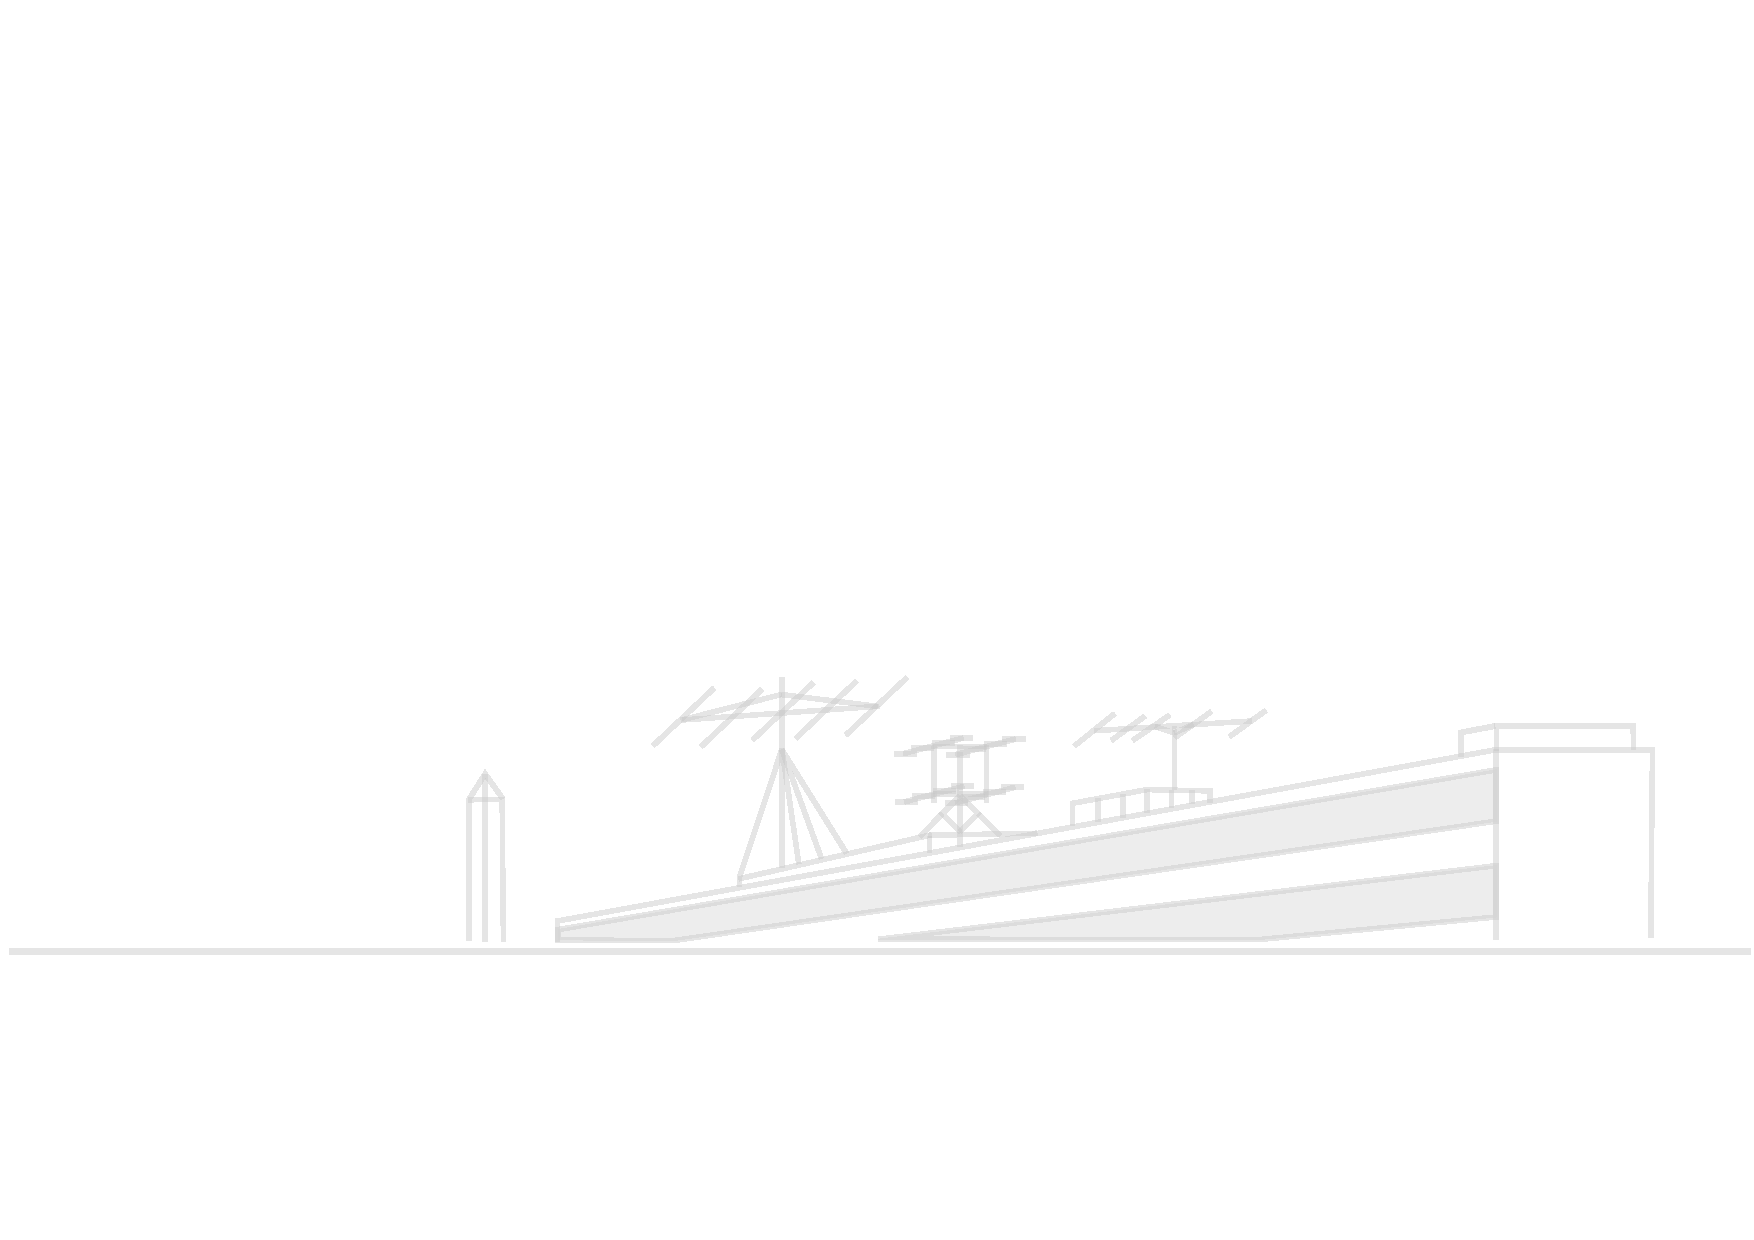
\includegraphics[width=17.8cm]{texdata/dk0tu_rooftop_background.pdf}
}

% Foliennummer einfügen
\setbeamertemplate{footline}[frame number]
%\setbeamertemplate{footline}{}

% Ändere das Zeichen vor jedem item
%\setbeamertemplate{itemize item}{\color{craneorange}$\blacktriangleright$}
%\setbeamertemplate{itemize subitem}{\color{craneorange}$\triangleright$}
%\setbeamertemplate{itemize subsubitem}{\color{craneorange}$\blacktriangleright$}

% Ändert die Blöcke 
\setbeamertemplate{blocks}[rounded][shadow=true]
% default | rounded [shadow=true|false]

%
% Eigene Kommandos
%

% Hack to get natbib and beamer working together. "The beamer user guide suggests
% that only the manual bibliography entry approach is supported"
% on some system it works out of the box, sometimes you need the hack :-(
% so check it --dl7bst
\ifdefined\newblock
    \relax
\else
    \newcommand{\newblock}{}
\fi

% \includedia command to generate png out of a dia file
% NEEDS installed dia and pdflatex option --shell-escape
\newcommand{\includedia}[1]{
    \immediate\write18{/usr/bin/dia #1.dia -e #1_diatmp.png -t png}
}

% RICHIG GROSSER FONT!
\newfont{\bigfont}{cmr10 at 144pt}
\newfont{\smallfont}{cmr10 at 8pt}

% Römische Ziffern
\makeatletter
\newcommand{\rmnum}[1]{\romannumeral #1}
\newcommand{\Rmnum}[1]{\expandafter\@slowromancap\romannumeral #1@}
\makeatother

% Schwarze Überschrift
%\setbeamercolor{frametitle}{fg=black}
%\setbeamercolor{title}{fg=black}

% Item- und Box-Farben
\definecolor{deepBlue}{HTML}{000066}
\setbeamercolor{itemize item}{fg=deepBlue}
\setbeamercolor{itemize subitem}{fg=deepBlue}
\setbeamercolor{description item}{fg=deepBlue}
\setbeamercolor{block title}{fg=deepBlue!100, bg=blue!15}
\setbeamercolor{block body}{fg=black, bg=blue!5}
\setbeamercolor{block title alerted}{fg=deepBlue, bg=red!75}
\setbeamercolor{block body alerted}{fg=black, bg=red!15}
\setbeamercolor*{block title example}{fg=blue!50, bg=blue!10}
\setbeamercolor*{block body example}{fg= blue, bg=blue!5}

%\setbeamercolor{section in head/foot}{parent=palette primary}
%\setbeamercolor{subsection in head/foot}{parent=palette secondary}
%\setbeamercolor{sidebar}{fg=darkblue,bg=yellow!90!orange}
%\setbeamercolor{title in sidebar}{fg=darkblue}
%\setbeamercolor{author in sidebar}{fg=darkblue}
%\setbeamercolor{section in sidebar}{fg=darkblue!10!black}
%\setbeamercolor{subsection in sidebar}{fg=darkblue!50!black}

% Titlepage Infos
\title{AFu-Kurs nach DJ4UF}
\author[DKØTU]{DKØTU\\ \footnotesize{Amateurfunkgruppe der TU Berlin}}
\institute[DKØTU]{\url{http://www.dk0tu.de} }

% PDF-Eigenschaften
\subject{DK0TU-Amateurfunkkurs nach DJ4UF}
\keywords{Amateurfunk Kurs HAM Radio Course CC-BY-NC-SA OpenSource TU Berlin DK0TU}

\subtitle{Technik A 16: \\
          Messtechnik \\[2em]}
\date{Stand 26.05.2016}
 \begin{document}

\begin{frame}
    \titlepage
    \vfill
    \begin{center}
        \ccbyncsaeu\\
        {\tiny This work is licensed under the \em{Creative Commons Attribution-NonCommercial-ShareAlike 3.0 License}.}\\[0.5ex]
         \tiny Amateurfunkgruppe der Technische Universität Berlin (AfuTUB), DKØTU
         %\includegraphics[scale=0.5]{img/DK0TU_Logo.pdf}
    \end{center}
\end{frame}


%fixme Referenzen/Fußnoten-Systematik vereinheitlichen

\section*{Einleitung}

\begin{frame}
    \frametitle{Messgeräte}
    {\Large Was wisst ihr noch aus Kapitel \emph{E17}?}
\end{frame}

\begin{frame}
  \frametitle{Stehwellenmessgerät}
  \begin{center}
    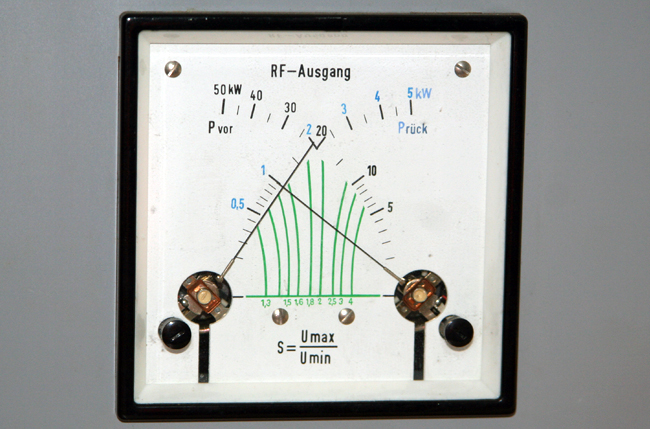
\includegraphics[width=1\textwidth,height=.8\textheight,keepaspectratio]{a16/RS_SWR.jpg}\\
    {\tiny SWR-Meter zum messen des Stehwellenverhältnisses \hyperlink{refs}{\cite{wmen}}}
  \end{center}
\end{frame}

\section*{Analog}

\begin{frame}
  \frametitle{Drehspulenmessgerät (Antik)}
  \begin{columns}
    \column{.3\textwidth}
    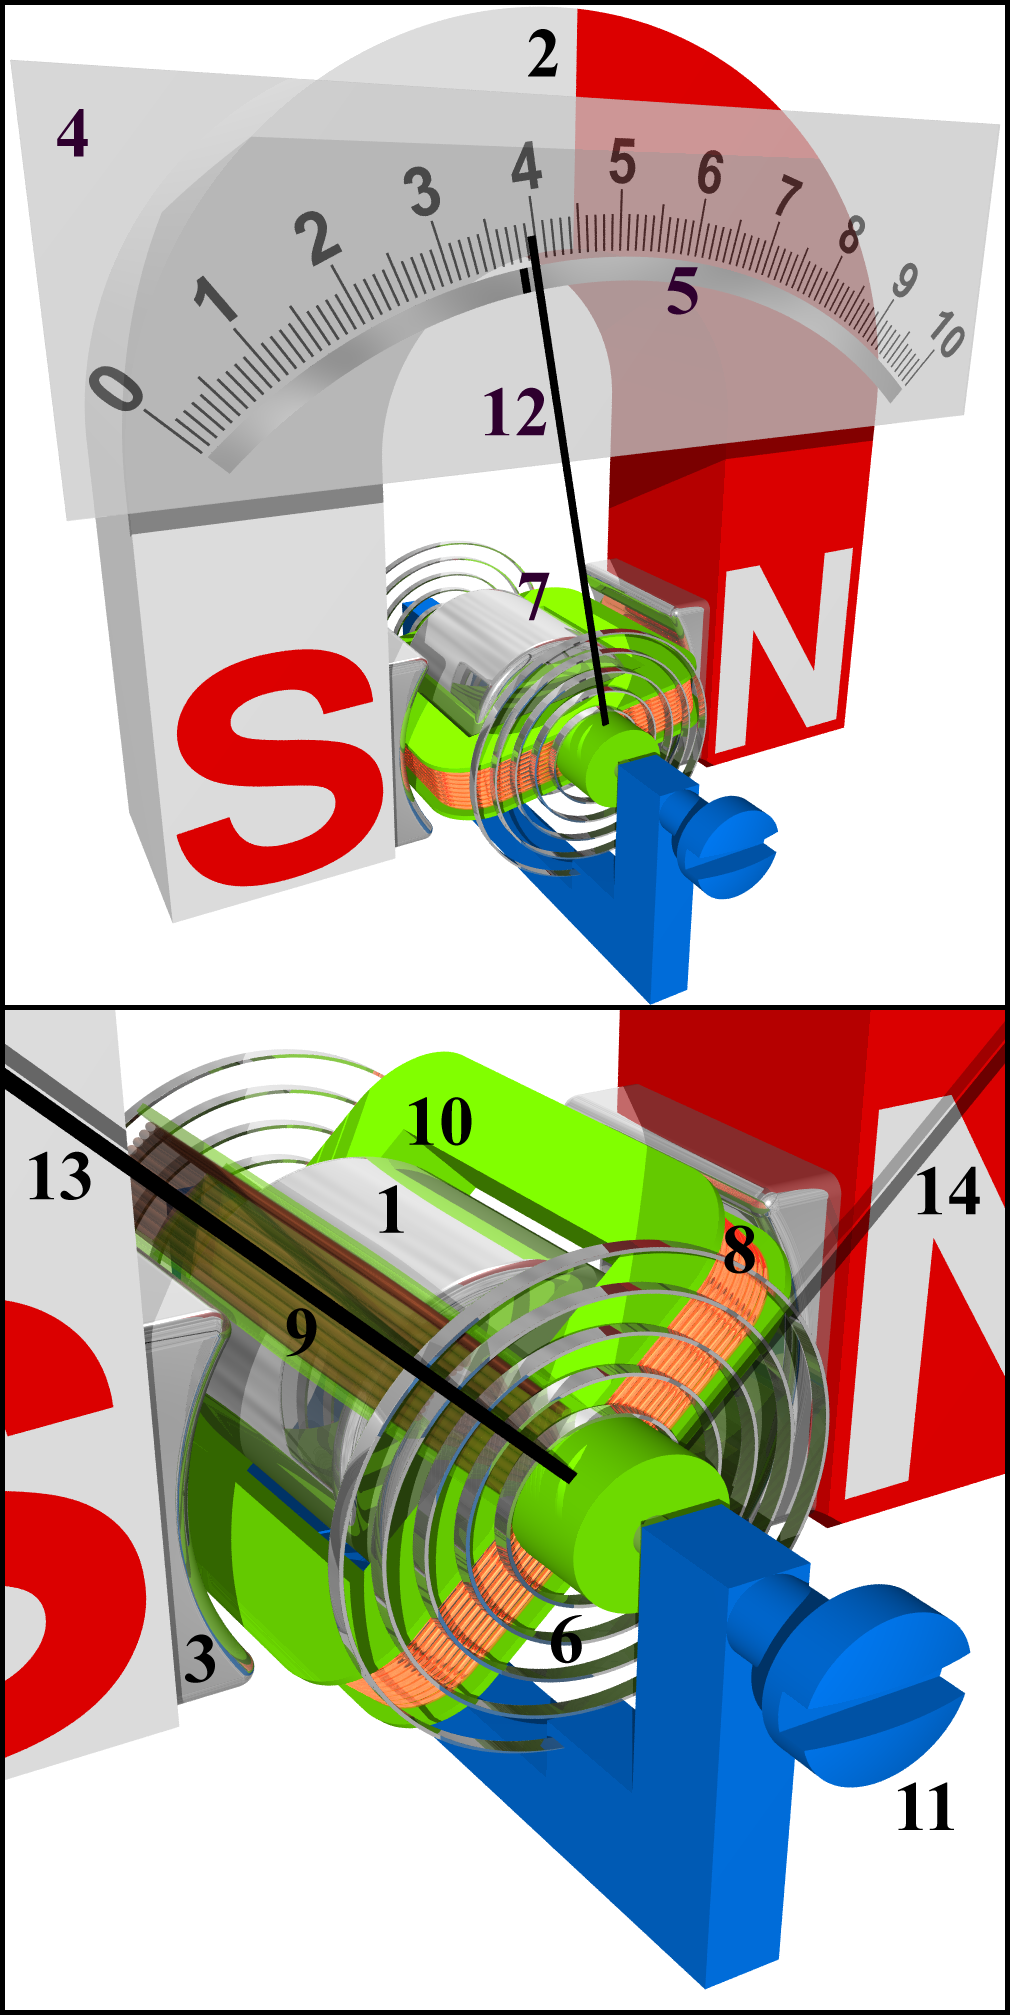
\includegraphics[width=.95\textwidth,height=.8\textheight,keepaspectratio]{a16/drehspulenMess.png}\\
    {\tiny Prinzip Drehspulenmessgerät \href{refs}{\cite{wmen}}}
    \column{.65\textwidth}
    \begin{footnotesize}
      \begin{enumerate}
        \item Weicheisenkern der Drehspule
        \item Permanentmagnet
        \item Polschuh zur Bündelung des Magnetfeldes
        \item Skala
        \item Hilfsspiegel zur genauen Ablesung
        \item Rückstellfeder
        \item Drehspule
        \item Drehspule in Nulllage
        \item Drehspule bei Maximalausschlag
        \item Joch der Spule
        \item Stellschraube für Nullpunkteinstellung
        \item Zeiger
        \item Zeiger in Nulllage
        \item Zeiger bei Maximalausschlag
      \end{enumerate}
    \end{footnotesize}
  \end{columns}
\end{frame}

\begin{frame}
  \frametitle{Funktionsprinzip analoger Messgeräte}
  \begin{itemize}
    \item Analoge Messgeräte funktionieren nach dem elektrodynamischen, oder dem elektrostatischen Prinzip
    \item Dabei erzeugt die zu messende Größe ein mechanisches Drehmoment zwischen dem feststehendem Messwerk und dem beweglichen Organ
    \item Die Empfindlichkeit wird in $k \Omega /V$ angegeben
    \item Für Gleichspannung sollte die Empfindlichkeit bei mindestens $20 k \Omega / V$ liegen
  \end{itemize}
\end{frame}

\begin{frame}
  %\frametitle{Symbole auf analogen Messgeräten}
  \begin{center}
    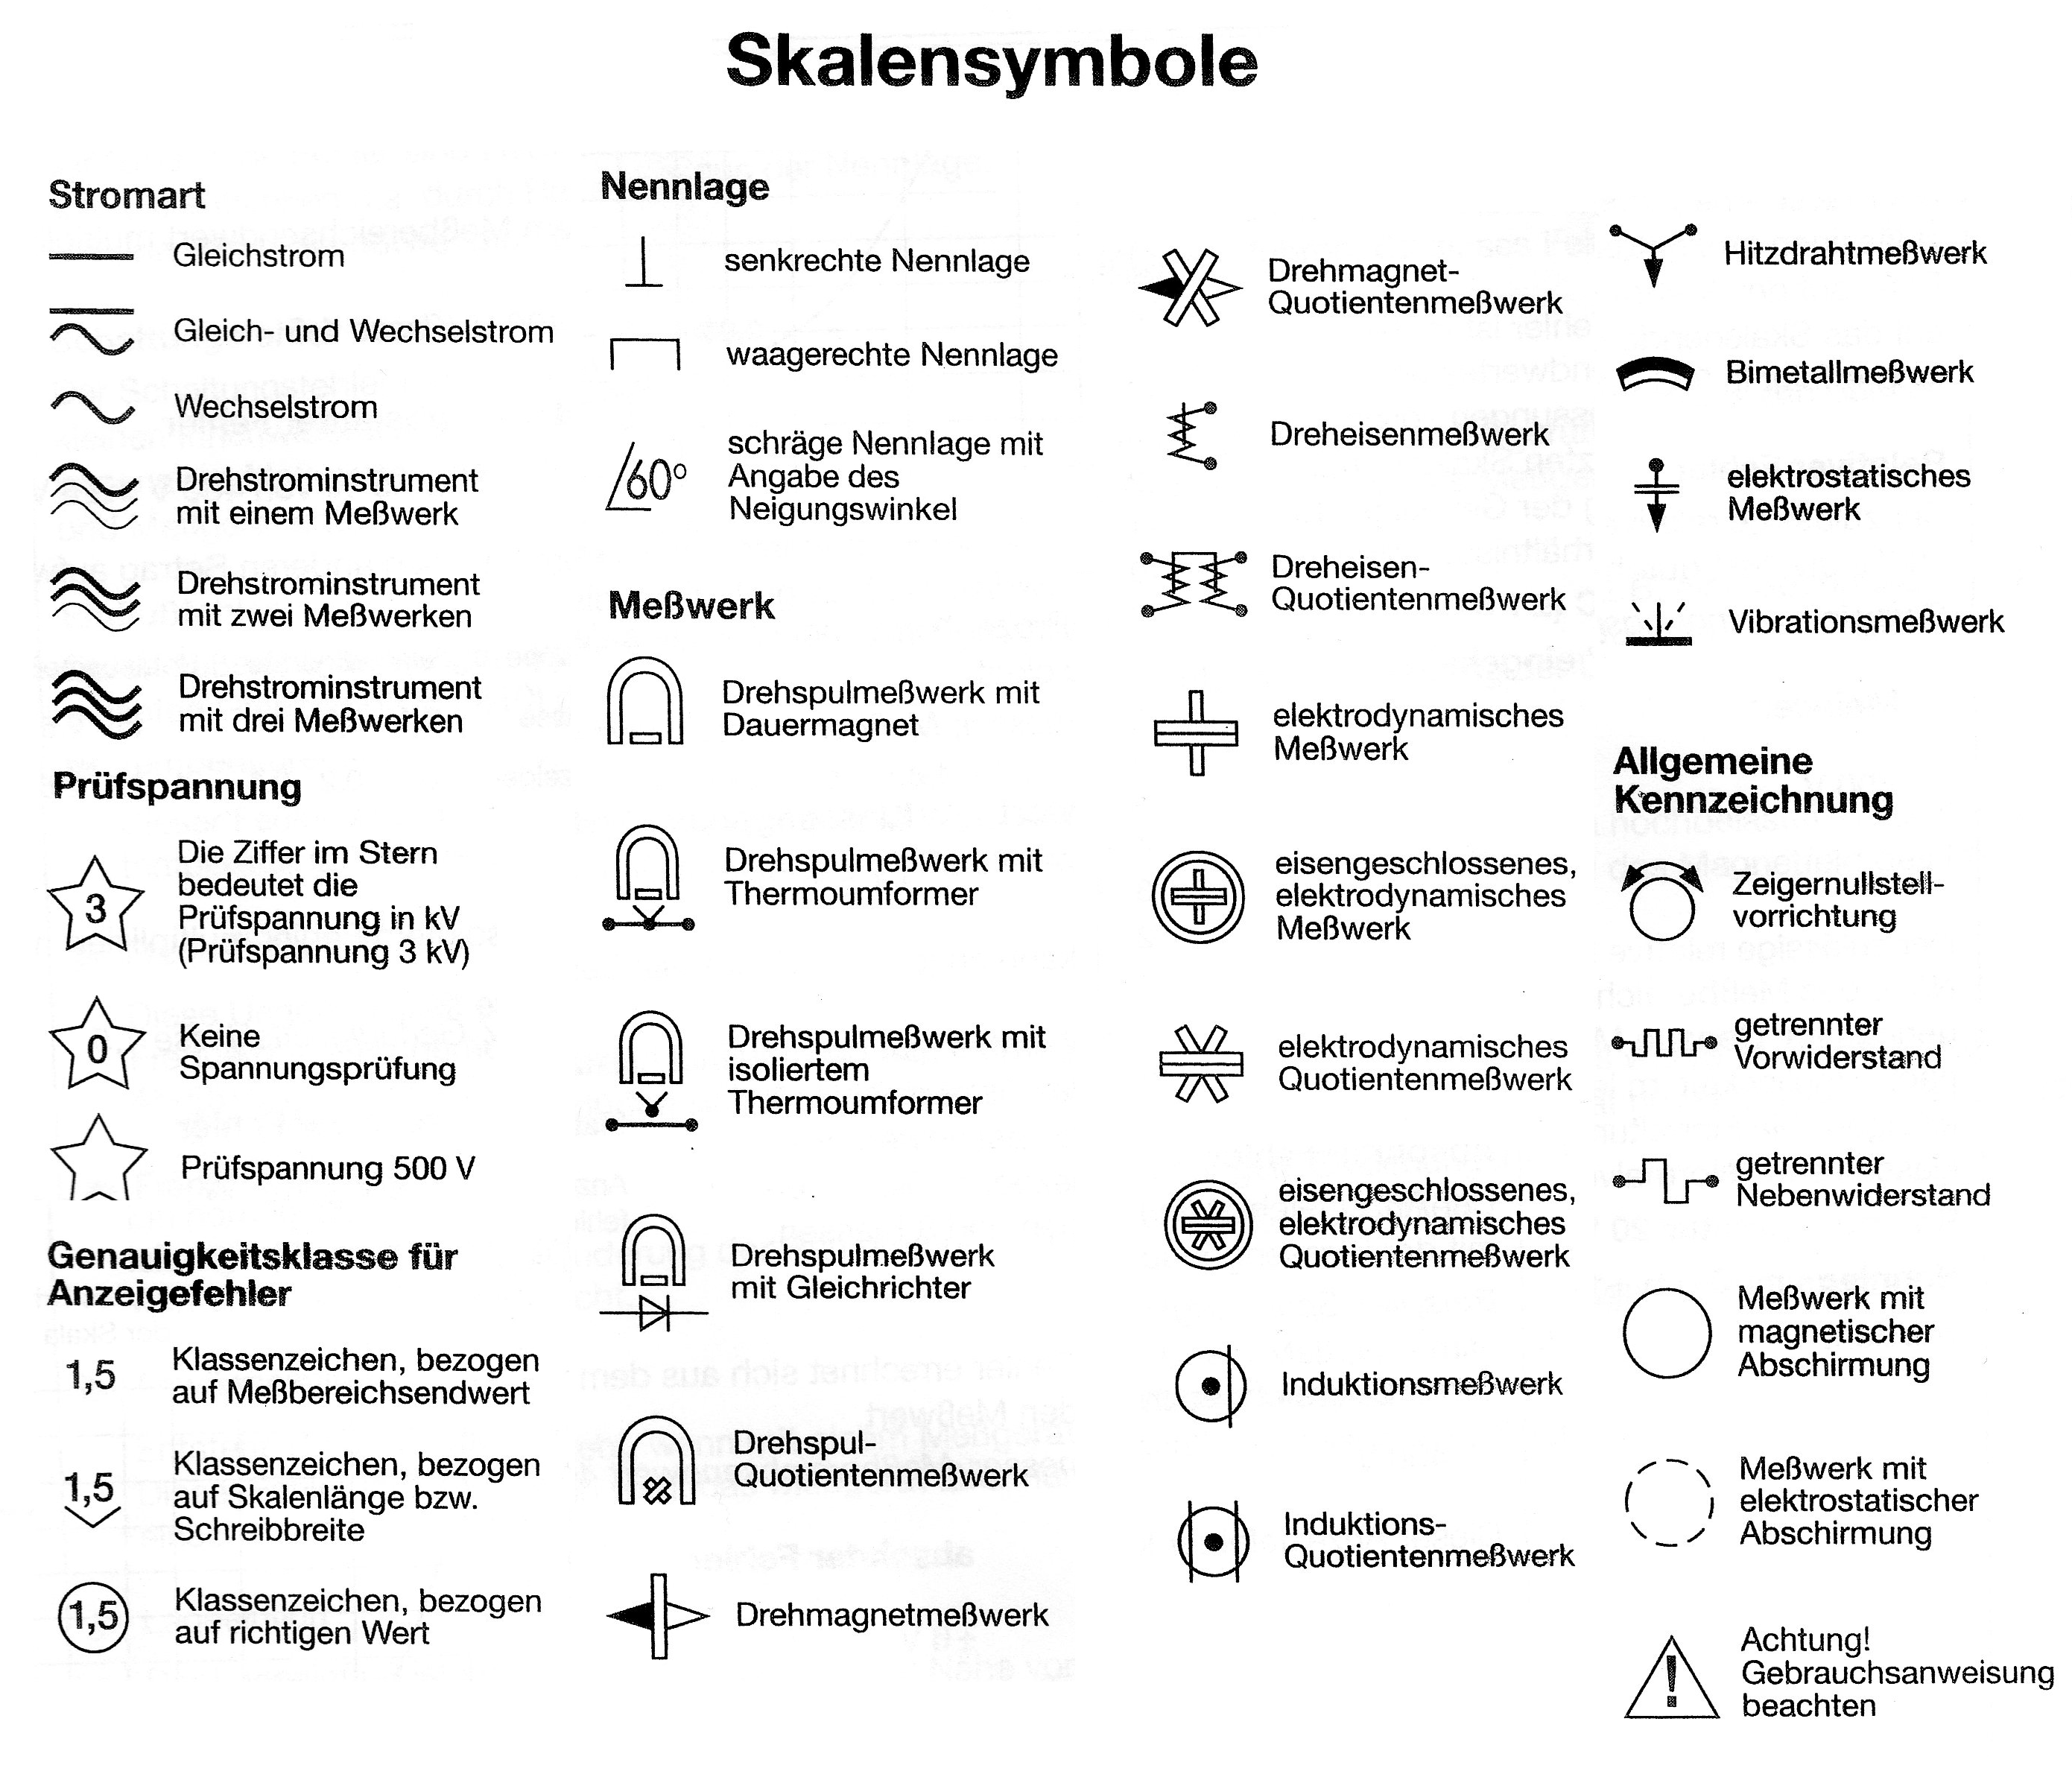
\includegraphics[width=\textwidth,height=\textheight,keepaspectratio]{a16/Symbole.png}
  \end{center}
\end{frame}

\begin{frame}
  \frametitle{Messgeräteklassen}
  Klasse gibt den prozentualen Fehler bezogen auf den Skalenendwert an
  \begin{center}
    \begin{tabular}{c|c}
      \textbf{Feinmessgeräte} & \textbf{Betriebsmessgeräte}\\ \hline
      Klasse 0,1 & Klasse 1,0 \\
      Klasse 0,2 & Klasse 1,5 \\
      Klasse 0,5 & Klasse 2,5 \\
      " " & Klasse 5,0 \\
    \end{tabular}
  \end{center}

  \pause

  \begin{exampleblock}{\textbf{TJ805} Mit einem Voltmeter der Klasse 1.5, das einen Skalenendwert von 300 Volt hat, messen Sie an einer Spannungsquelle 230 Volt. In welchem Bereich liegt der wahre Wert?}
    \only<2>{\vspace{1em}}
    \only<3>{Er liegt zwischen 225,5 und 234,5 Volt.}
  \end{exampleblock}
\end{frame}

\begin{frame}
  \frametitle{Messbereichserweiterung}
  \begin{columns}
    \column{.47\textwidth}
    \begin{center}
      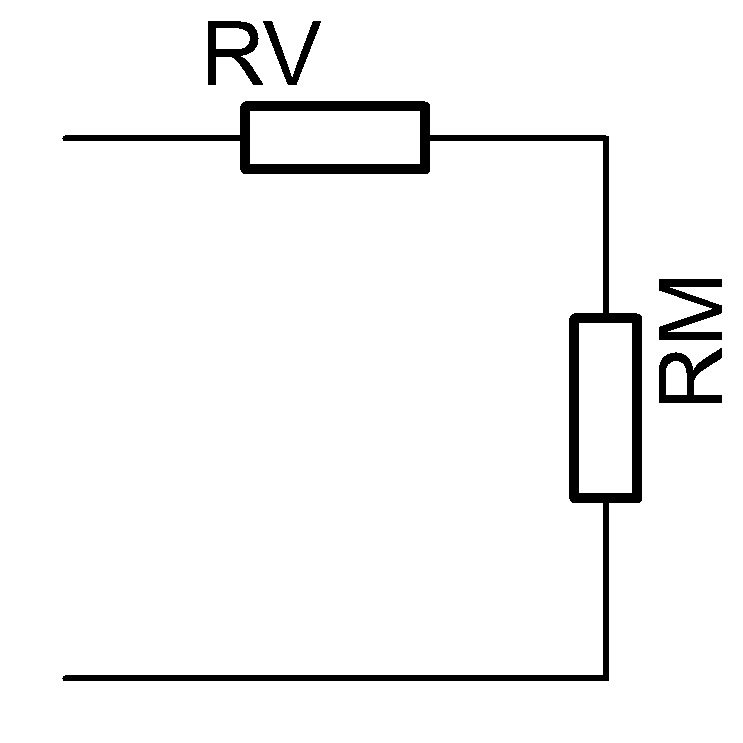
\includegraphics[width=\textwidth,height=.5\textheight,keepaspectratio]{a16/Messbereichserweiterung-Spannung.png}\\
      Spannungsmessgerät
    \end{center}
    \only<1>{\vspace{4em}}
    \only<2->{Zu große Spannung fällt am Vorwiderstand ab $\rightarrow$ Spannungsteiler \\
              (Messung höherer Spannungen möglich -- abhängig von $\frac{R_M}{R_{gesamt}}$)}
    \column{.47\textwidth}
    \begin{center}
      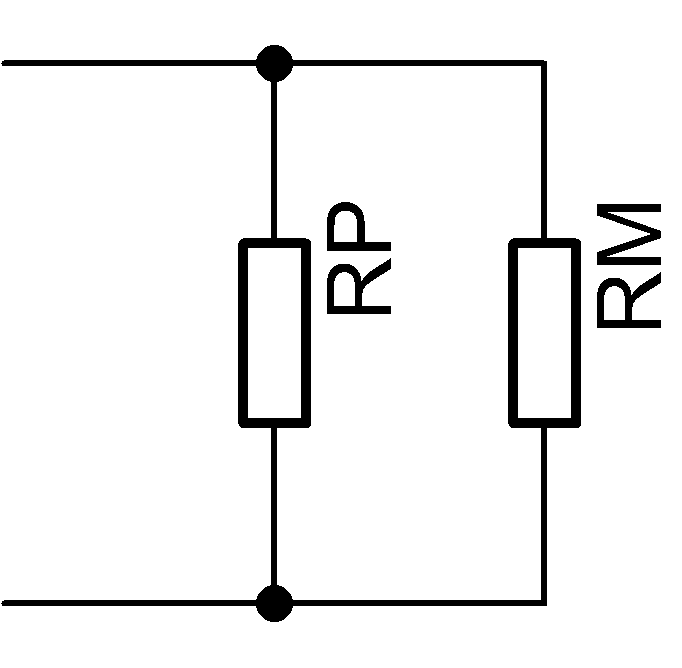
\includegraphics[width=\textwidth,height=.5\textheight,keepaspectratio]{a16/Messbereichserweiterung-Strom.png}\\
      Strommessgerät
    \end{center}
    \only<1-2>{\vspace{4em}}
    \only<3>{Zu großer Strom wird parallel durch einen Widerstand geleitet\vspace{2em}}
  \end{columns}
\end{frame}

\begin{frame}
  \frametitle{Messgleichrichter}
  \begin{columns}
    \column{.35\textwidth}
    \begin{center}
      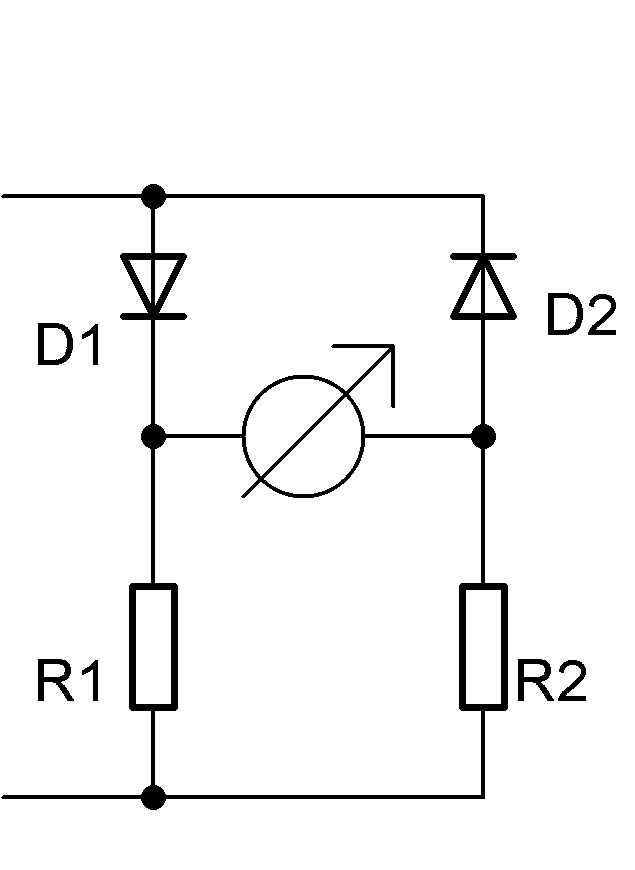
\includegraphics[width=\textwidth,height=.4\textheight,keepaspectratio]{a16/Messgleichrichter1.png}\\
      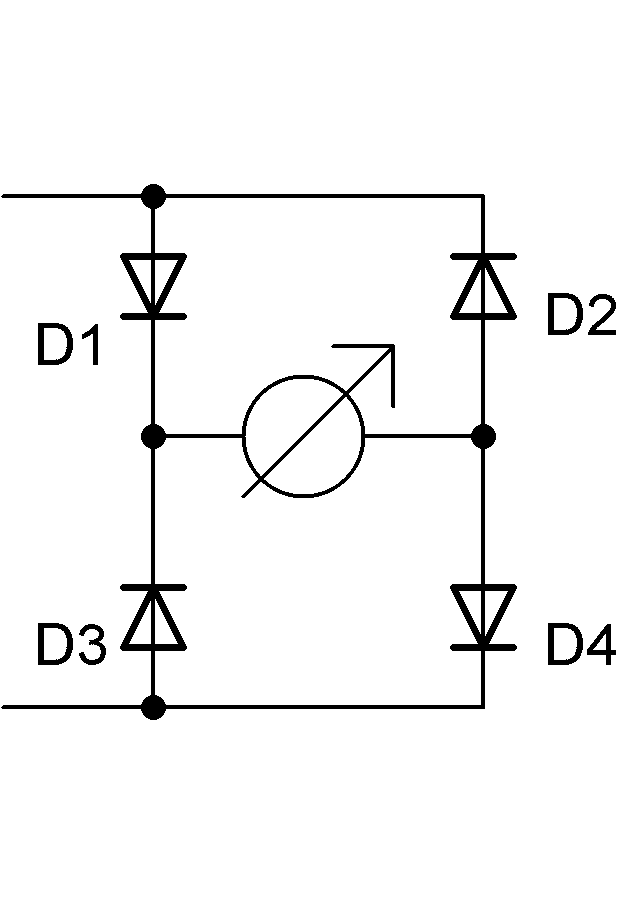
\includegraphics[width=\textwidth,height=.4\textheight,keepaspectratio]{a16/Messgleichrichter2.png}\\
      {\tiny Mögliche Schaltungen für Messgleichrichter}
    \end{center}
    \column{.65\textwidth}
    \begin{itemize}
      \item Drehspulmesswerke eignen sich nur zum messen von Gleichstrom
      \item Um auch Wechselspannungen messen zu können, nutzt man Messgleichrichter
      \item Diese funktionieren aber nur für sinusförmige Signale
      \item Für andere Signalformen gibt es das Dreheisenmesswerk
      \item Diese brauchen keinen Gleichrichter benötigen aber recht viel Leistung und sind nicht als Feinmessgeräte tauglich
      \item Will man im GHz-Bereich messen, benötigt man einen speziellen Thermoumformer
    \end{itemize}
  \end{columns}
\end{frame}

\section*{Digital}

\begin{frame}
  \frametitle{Digitales Multimeter}
  \begin{columns}
    \column{.3\textwidth}
    \begin{center}
      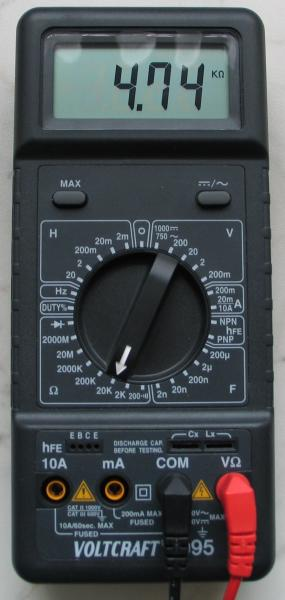
\includegraphics[width=\textwidth,height=.8\textheight,keepaspectratio]{a16/digitalmultimeter.jpg}\\
      {\tiny Digitales Multimeter (DMM) \href{refs}{\cite{wmde}}}
    \end{center}
    \column{.65\textwidth}
    \begin{itemize}
      \item Verringern Gefahr von Ablesefehlern
      \item Brauchen Strom zum messen
      \item Auflösung ist die kleinste Einteilung der Anzeige
      \item Neben Auflösung auch Genauigkeit beachten
      \item Einfache DMM messen:\newline Spannung, Stromstärke, Widerstand
      \item Bessere:\newline Durchgangsprüfung (auf Geschwindigkeit achten!), Kapazität, (niedrige) Frequenzen, Dioden- und Transistortest
      \item Selten auch:\newline Induktivität, Temperatur, Temperatur, Verstärkung von Bipolartransistoren, Lichtstärke, Schalldruck
    \end{itemize}
  \end{columns}
\end{frame}

\begin{frame}
  \frametitle{Was wo anschließen?}
  \begin{columns}
    \column{.32\textwidth}
    \begin{center}
      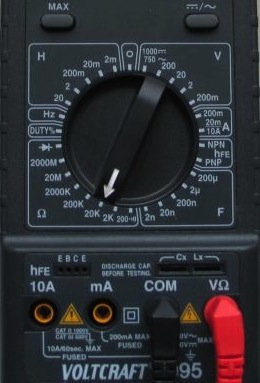
\includegraphics[width=\textwidth,height=.8\textheight,keepaspectratio]{a16/digitalmultimeterMess.jpg}\\
      {\tiny Wählrad und Anschlüsse eines Multimeters \href{refs}{\cite{wmde}}}
    \end{center}
    \column{.65\textwidth}
    \begin{itemize}
      \item Was kann alles gemessen werden?
      \item Wo anschließen zum Strom messen?
      \item Wo anschließen zum Spannung messen?
      \item Welcher Messbereich?
    \end{itemize}
  \end{columns}
\end{frame}

\begin{frame}
  \frametitle{Messfehler}
  \begin{center}
    \begin{tabular}{ccc}
      Nullpunktabweichung & Empfindlichkeitsabweichung & Linearitätsabweichung
    \end{tabular}
    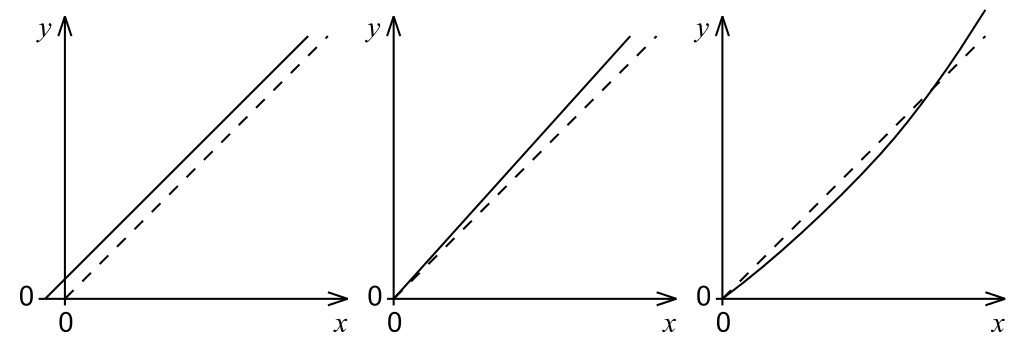
\includegraphics[width=1\textwidth,height=.6\textheight]{a16/werMisstMisst.png}\\
    {\tiny Mögliche Abweichungen durch Messsfehler \href{refs}{\cite{wmde}}}
  \end{center}
\end{frame}

\section*{Oszilloskop}


\begin{frame}
  \frametitle{Oszilloskop}
  \begin{center}
    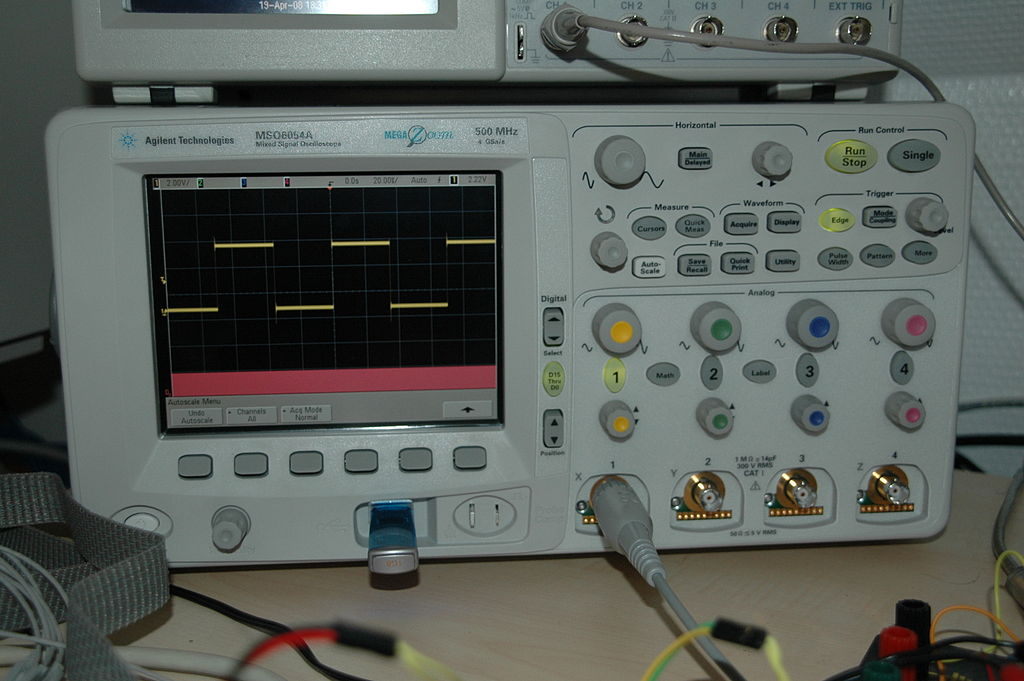
\includegraphics[width=1\textwidth,height=.8\textheight,keepaspectratio]{a16/osziModern.jpg}\\
    {\tiny Modernes Speicheroszilloskop \href{refs}{\cite{wmde}}}
  \end{center}
\end{frame}

\begin{frame}
  \frametitle{Oszilloskop}
  \begin{itemize}
    \item Können zeitliche Verläufe von Spannungen darstellen
    \item Anzeige mit Elektronenstrahlröhre (ein Strahl, sehr genau, direkte Spannungsumsetzung) oder LCD (moderner, Computer-Schaltung bereitet das Bild auf)
    \item Kann stehende Bilder von Wellen darstellen, indem die Welle immer an einem bestimmten Amplitudenwert getriggert (gestartet) wird
    \item Benötigt dafür eine Triggereinrichtung
  \end{itemize}
\end{frame}

\begin{frame}
  \frametitle{Oszilloskop}
  \begin{center}
    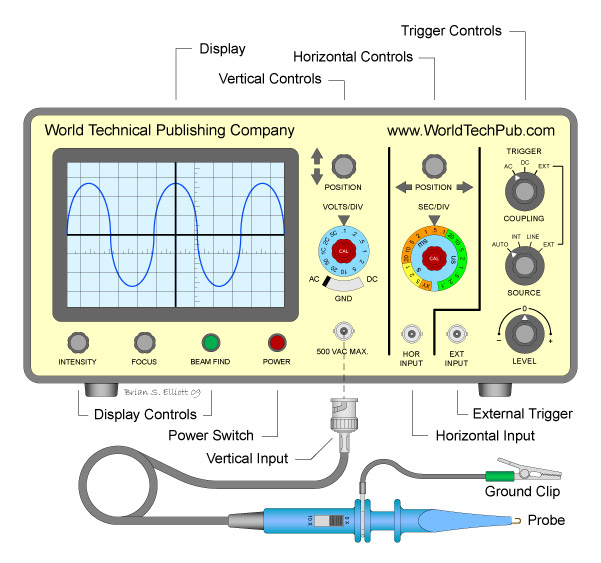
\includegraphics[width=.8\textwidth,height=.8\textheight,keepaspectratio]{e17/WTPCOscilloscopeBeschreiben.jpg}\\
    {\tiny Anschlüsse und Schalter eines Oszilloskops \href{refs}{\cite{wmen}}}
  \end{center}
\end{frame}

\begin{frame}
  \frametitle{Oszilloskop ablesen}
  \begin{center}
    $100mV / Div$ und $0,1ms / Div$\\
    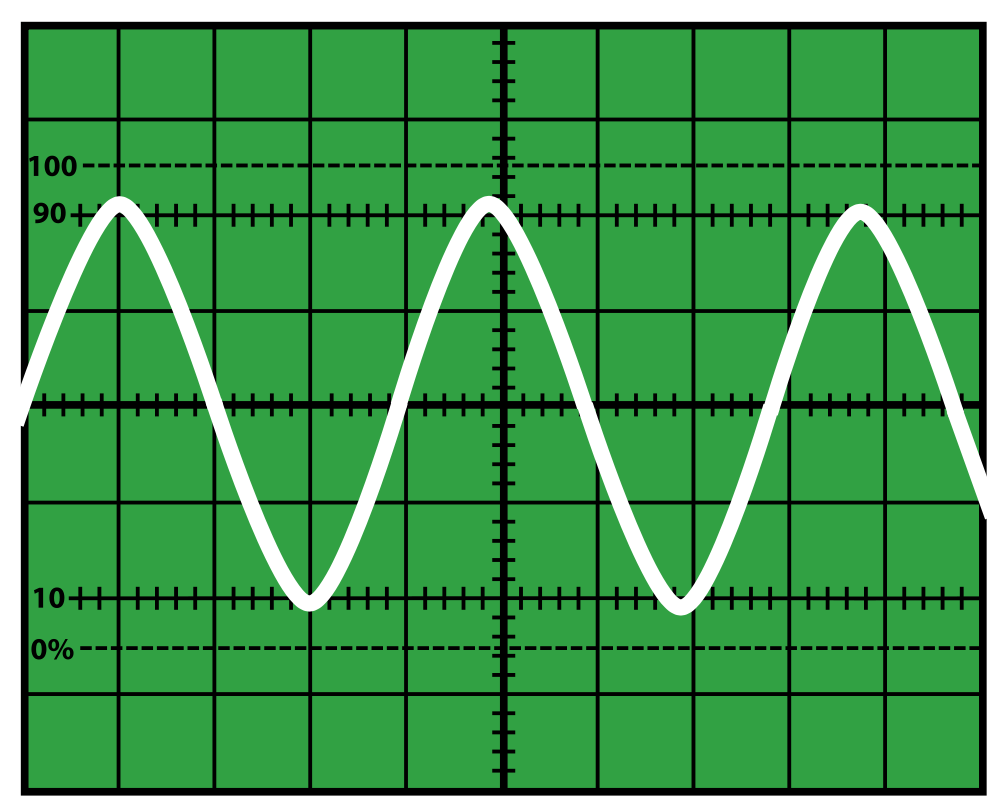
\includegraphics[width=.8\textwidth,height=.7\textheight,keepaspectratio]{a16/OsziTon.png}\\
    {\tiny Signal auf einem Oszilloskop \href{refs}{\cite{wmde}}}
  \end{center}
\end{frame}

\begin{frame}
  \frametitle{Verschiedene Signalformen}
  \begin{center}
    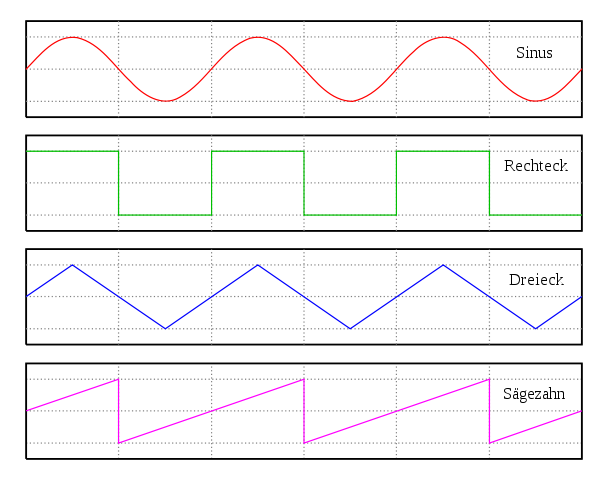
\includegraphics[width=0.95\textwidth,height=.8\textheight,keepaspectratio]{a16/Signalformen.png}\\
    {\tiny Verschiedene elementare Signalformen \href{refs}{\cite{wmen}}}
  \end{center}
\end{frame}

\begin{frame}
  \frametitle{Spannungen}
  \begin{center}
    \begin{itemize}
      \item Peak-to-Peak
      \item RMS (root mean square) -- Effektivwert
      \item Bei Sinus: $u_{Spitze} = \sqrt{2} \cdot U_{eff}$ \\
    \end{itemize}
  \end{center}
  \begin{exampleblock}{Aufgabe}
    Berechnet die Spitze-Spitze-Spannung der in Europa üblichen Netzspannung!
  \end{exampleblock}
\end{frame}

\section*{Absorptions"-frequenz"-messgerät}
\begin{frame}
  \frametitle{Absorptionsfrequenzmessgerät}
  \begin{columns}
    \column{.6\textwidth}
    \begin{center}
      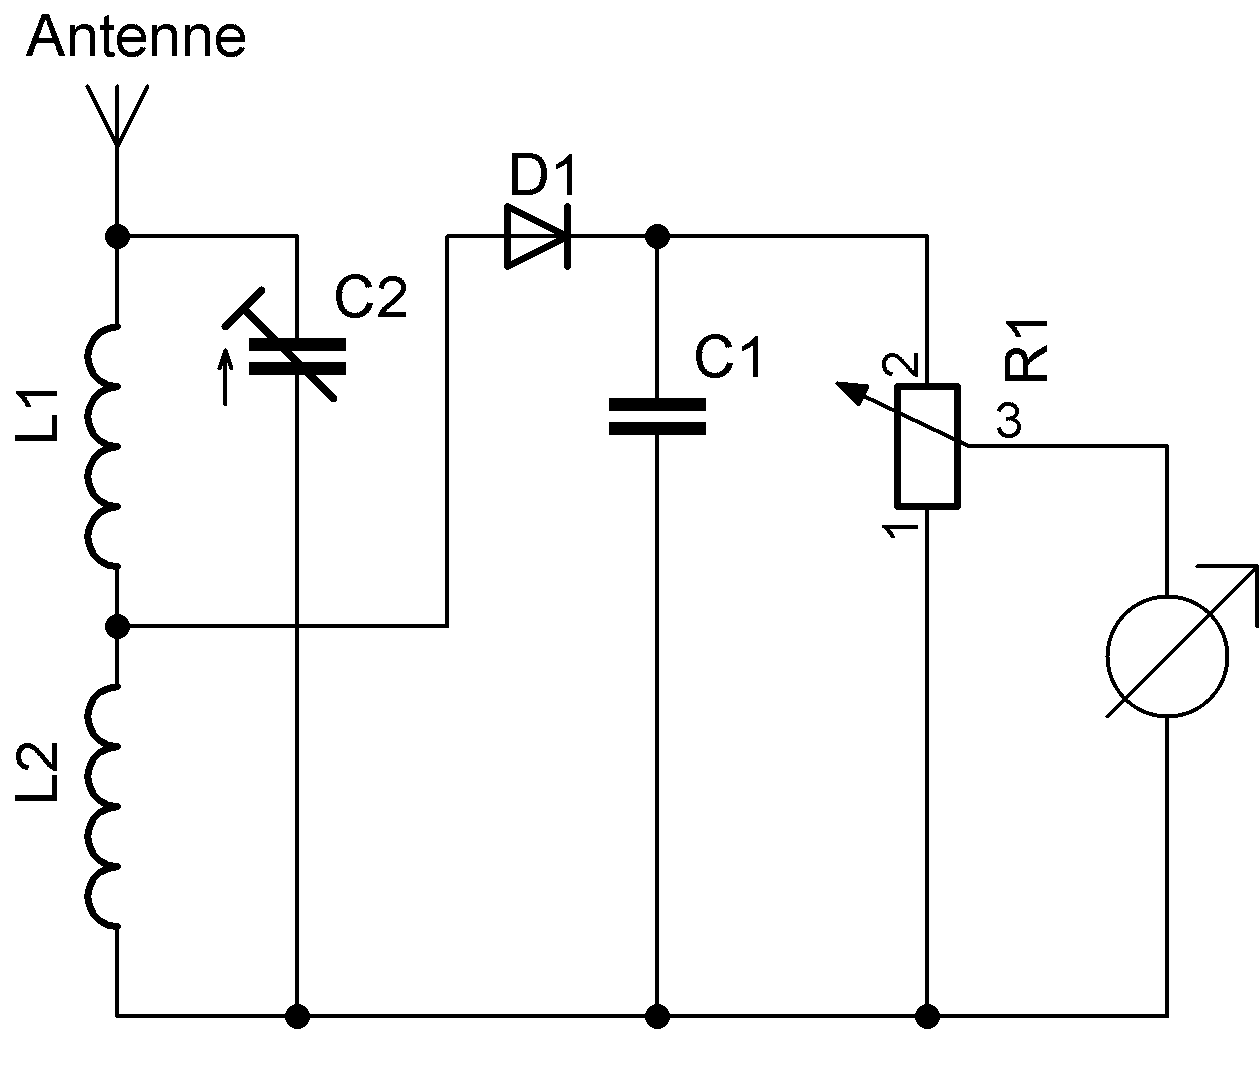
\includegraphics[width=\textwidth,height=.8\textheight,keepaspectratio]{a16/Absorptionsfrequenzmesser.png}\\
      {\tiny Schaltung eines Absorptionsfrequenzmessgeräts}
    \end{center}
    \column{.4\textwidth}
    \begin{itemize}
      \item Besteht aus einer Antenne, einem passiven Schwingkreis hoher Güte und  einem AM-Demodulator
      \item Damit lassen sich passiv Senderfrequenzen und Oberwellen feststellen
      \item Anzeigegenauigkeit liegt bei etwa 5\%
    \end{itemize}
  \end{columns}
\end{frame}

\section*{Feld"-stärke"-anzeiger}
\begin{frame}
  \frametitle{Feldstärkeanzeiger}
  \begin{columns}
    \column{.6\textwidth}
    \begin{center}
      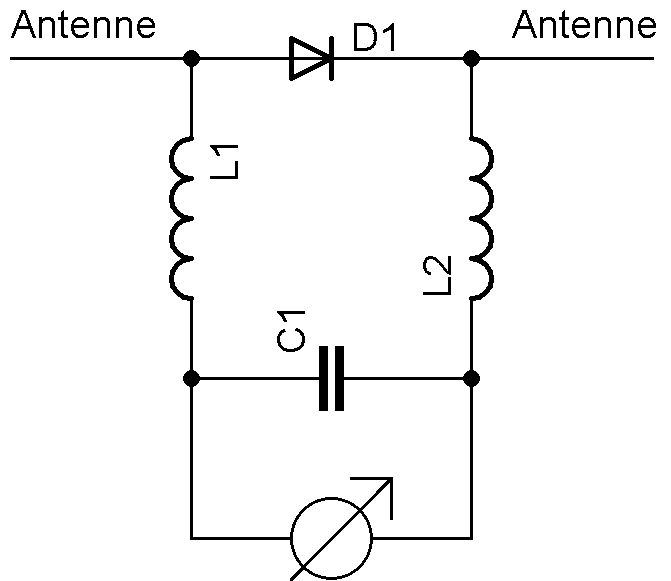
\includegraphics[width=\textwidth,height=.8\textheight,keepaspectratio]{a16/Feldstaerkeanzeiger.png}\\
      {\tiny Schaltung eines Feldstärkeanzeigers (nach Prüfungsfrage TJ706)}
    \end{center}
    \column{.4\textwidth}
    \begin{itemize}
      \item Wird zum Prüfen (\emph{nicht zum Messen!}) der Feldstärke genutzt
      \item Besteht aus einer HF-Diode, HF-Drosseln und einem Kondensator
    \end{itemize}
    \begin{flushright}
      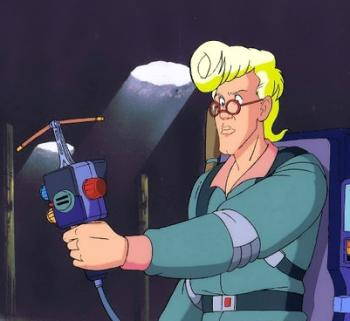
\includegraphics[width=.7\textwidth,keepaspectratio]{a16/ghostbusters_egon.jpg}\\
      {\tiny http://tvtropes.org (cc-nc-sa 3.0)}
    \end{flushright}
  \end{columns}
\end{frame}

\section*{Dipmeter}

\begin{frame}
  \frametitle{Dipmeter}
  \begin{columns}
    \column{.35\textwidth}
    \begin{center}
      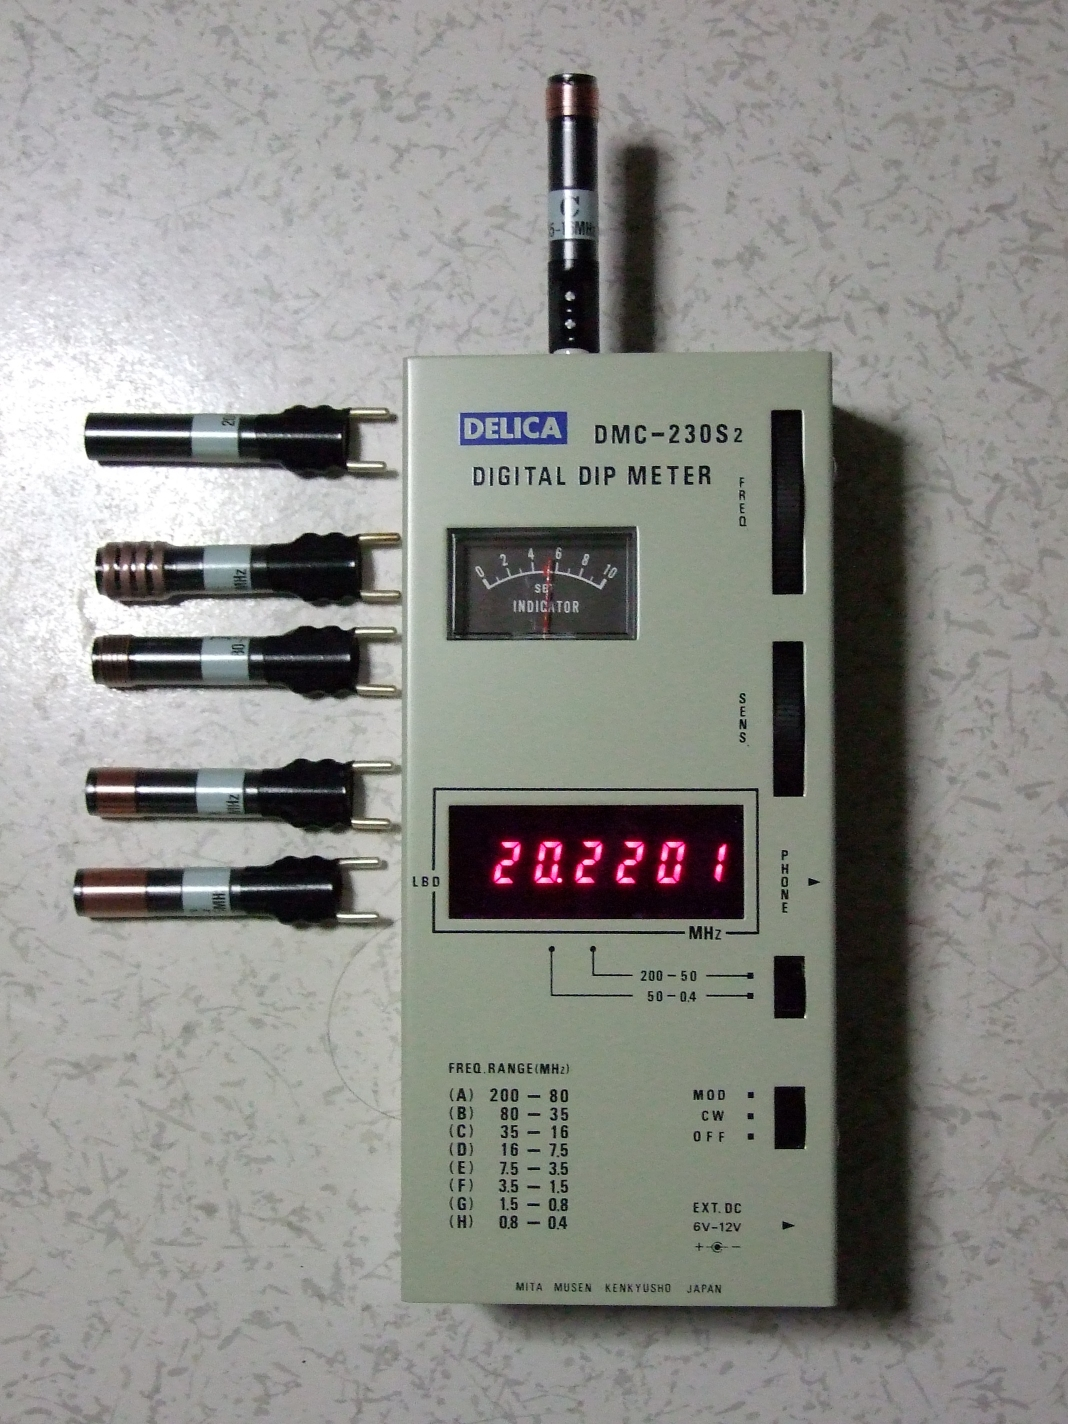
\includegraphics[width=\textwidth,height=.8\textheight,keepaspectratio]{a16/Dipmeter.jpg}\\
      {\tiny Dipmeter mit beiliegenden Mess-Spulen \href{refs}{\cite{wmen}}}
    \end{center}
    \column{.65\textwidth}
    \begin{itemize}
      \item prinzipiell ein Oszillator mit nach außen geführter Schwingkreisspule
      \item Schwingkreis wird durch das Messobjekt beeinflusst
      \item Rückgang der Schwingungsamplitude wird mit einer Anzeige sichtbar gemacht
      \item Anzeigegenauigkeit liegt bei etwa 10\%
      \item kann indirekt eine Induktivität messen $\rightarrow$ Kondensator parallel zur Induktivität schalten, Resonanzfrequenz ermitteln und umrechnen
      \item zum Messen wird eine relativ lose Kopplung zwischen Dipmeter und Messobjekt benötigt, da sonst das Messobjekt verstimmt wird und das Messergebnis dadurch verfälscht
    \end{itemize}
  \end{columns}
\end{frame}

\section*{Frequenzzähler}

\begin{frame}
  \frametitle{Frequenzzähler}
  \begin{columns}
    \column{.4\textwidth}
    \begin{center}
      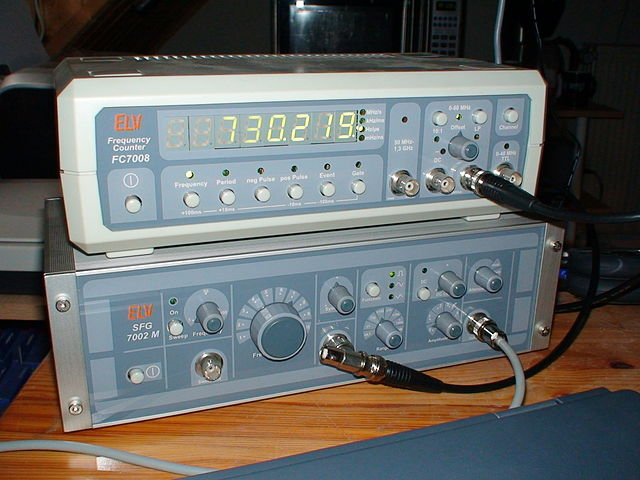
\includegraphics[width=\textwidth,height=.8\textheight,keepaspectratio]{a16/Frequenzzaehler.jpg}\\
      {\tiny Frequenzzähler von ELV \href{refs}{\cite{wmen}}}
    \end{center}
    \column{.6\textwidth}
    \begin{itemize}
      \item zählt während einer eingestellten Torzeit die ankommenden Impulse
      \item zur Erhöhung der Genauigkeit müssen mehr Impulse gezählt werden $\rightarrow$ längere Torzeit einstellen
      \item kann keine Oberwellen messen, wenn die Grundfrequenz noch vorhanden ist
      \item sehr genaue Messungen mit einer hohen Auflösung und einer temperaturstabilen Quarzzeitbasis möglich
      \item zum Messen von höheren Frequenzen einen Vorteiler verwenden $\rightarrow$ meistens Faktor 10
    \end{itemize}
  \end{columns}
\end{frame}

\section*{Spektrum"-analysator}
\begin{frame}
  \frametitle{Spektrumanalysator}
  \begin{columns}
    \column{.5\textwidth}
    \begin{center}
      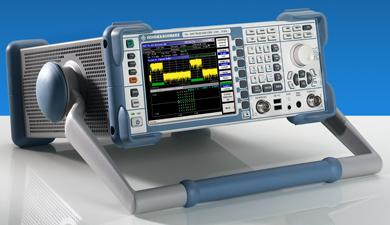
\includegraphics[width=\textwidth,height=.8\textheight,keepaspectratio]{a16/Spektrumanalysator.jpg}\\
      {\tiny Beispiel eines Spektrumanalysators \href{refs}{\cite{wp}}}
    \end{center}
    \column{.5\textwidth}
    \begin{itemize}
      \item kann die Amplitude eines Signals in Abhängigkeit der Frequenz darstellen
      \item besitzt dafür einen ``Wobbeloszillator'', der schnell seine Frequenz ändern kann
      \item Oberwellen mit sehr breiter Wobbelbandbreite messen
      \item Senderbandreite mit sehr schmaler Wobbelbandbreite messen
    \end{itemize}
  \end{columns}
\end{frame}

\begin{frame}
  \frametitle{Spektrumanalysator}
  \begin{center}
    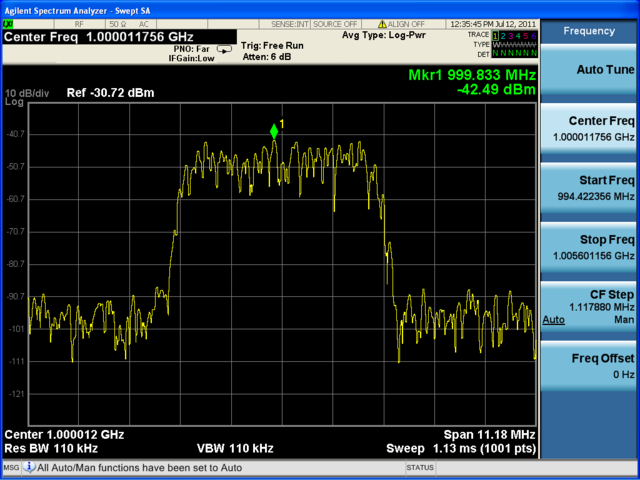
\includegraphics[width=\textwidth,height=.8\textheight,keepaspectratio]{a16/Spektrumanalysator-Display.png}\\
    {\tiny Display eines Spektrumanalysators zeigt Frequenzgang \href{refs}{\cite{wp}}}
  \end{center}
\end{frame}

\renewcommand{\refname}{Referenzen}

\hypertarget{refs}{}
\textcolor{white}{} \\ %\vspace{} geht nicht
\Large Referenzen/Links
\footnotesize

\begin{thebibliography}{}
  \bibitem{a17}  Moltrecht A 16: \\
    \url{https://www.darc.de/der-club/referate/ajw/lehrgang-ta/a16/}

  \bibitem{wp}    Wikipedia DE: \\
    \url{http://commons.wikimedia.org/wiki/File:FSL.jpg}\\
    \url{http://de.wikipedia.org/wiki/Datei:SpectrumAnalyzerDisplay.png}

  \bibitem{wmde} Wikimedia DE:\\
    \url{https://commons.wikimedia.org/wiki/File:Oszi_Ton.svg}\\
    \url{https://commons.wikimedia.org/wiki/File:Modernes_Speicheroszilloskop.jpg}\\
    \url{https://commons.wikimedia.org/wiki/File:AMT_Fehler.svg}\\
    \url{http://commons.wikimedia.org/wiki/File:Digitalmultimeter.jpg}\\

  \bibitem{wmen} Wikimedia EN:\\
    \url{https://commons.wikimedia.org/wiki/File:Dipmeter_and_its_probe_coils.jpg}\\
    \url{https://commons.wikimedia.org/wiki/File:RS_SWR.jpg}\\
    \url{https://commons.wikimedia.org/wiki/File:Moving_coil_instrument_principle.png}\\
    \url{http://commons.wikimedia.org/wiki/File:Waveforms_de.svg}
    \url{http://commons.wikimedia.org/wiki/File:Frequency_counter.JPG}\\
    \url{https://en.wikipedia.org/wiki/File:WTPC_Oscilloscope-1.jpg}\\

\end{thebibliography}

% Hier könnte noch eine Kontaktfolie stehen

\end{document}

